%%%%%%%%%%%%%%%%%%%%%%%%%%%
% PREAMBOLO DEL DOCUMENTO %
%%%%%%%%%%%%%%%%%%%%%%%%%%%
\documentclass[a4paper,11pt,oneside,top=3cm,bottom=3cm,left=3.5cm,right=3.5cm,openright,reqno,table]{book}

% openany - fa iniziare i capitoli direttamente nella pagina successiva
% openright - fa iniziare i capitoli nella prima pagina destra disponibile 
% fleqn  - allinea le formule a sinistra anzichè centrarle
% leqno - dispone la numerazione delle formule sulla sinistra o destra
% reqno - dispone la numerazione delle formule sulla destra
%
\usepackage{packages}
% Per non appesantire troppo questo file
% quasi tutti i pacchetti usati sono salvati in packages.sty
%
\linespread{1.5}
% Per avere la parola BOZZA scritta su tutte le pagine

% funziona solo in modalità PS
% Invece per i PDF ho risolto così:
% pdftk tesi.pdf background bozza.pdf output tesi_bozza.pdf
%
%%%%%%%%%%%%%%%%%%%%%%%%%%%%%%%%%
%   DOCUMENTO VERO E PROPRIO    %
%%%%%%%%%%%%%%%%%%%%%%%%%%%%%%%%%
\begin{document}
% FRONTESPIZIO %
\begin{titlepage}
\changepage{}{}{}{-7.5 mm}{}{}{}{}{}
% parametri per cambiare le dimensioni di una singola pagina in ordine:
% {textheight}{textwidth}{evensidemargin}{oddsidemargin}{columnsep}
% {topmargin}{headheight}{headsep}{footskip}
% se voglio centrare la pagina devo mettere bindingoffset/2
% i primi 5 parametri posso usarli con \changetext


\begin{center}

\includegraphics [width=.15\columnwidth, angle=0]{unisa}\\ % height
\vspace{0.5cm}
{\LARGE \scshape Università degli Studi di Salerno}\\
\vspace{0.5cm}
{\Large Dipartimento di Informatica}\\
\vspace{0.1cm}
{\large Corso di Laurea Magistrale in Informatica}\\
\vspace{1.5cm}
{\Large \scshape Corso di Penetration Testing\\ and Ethical Hacking} \\
\vspace{4cm}
{\Huge \bfseries De-ICE S1.140} \\
\vspace{5cm}

\begin{minipage}[t]{7cm}
\flushleft
\textsc{Studente}

Lorenzo Criscuolo \\
Matricola: 0522501268
\end{minipage}
\hfill
\begin{minipage}[t]{7cm}
\flushright
\textsc{Docente}

Prof. \textbf{Arcangelo Castiglione} \\
{\small Università degli studi di Salerno} \\[0.25cm]
\end{minipage}

\vspace{3cm}

{\small Anno Accademico 2022-2023} %\\
%

%
\end{center}

\end{titlepage}
%

\frontmatter
% quello che segue è in numerazione romana e i capitoli non verranno numerati
% se non si vuole che compaia il numero di pagina basta usare il comando:
%\nonumber

% SOMMARIO %
\cleardoublepage
\include{frontmatter/sommario}
% INDICI %
\phantomsection
\addcontentsline{toc}{chapter}{Indice}
\tableofcontents
% Il simbolo * serve per evitare che comapaia nell'indice
\clearpage
%\listoffigures
%\clearpage
%\listoftables

\mainmatter
% quello che segue sarà in numerazione araba e i capitoli verranno numerati
%\part{Studio iniziale}
% CAPITOLI
\phantomsection
%\addcontentsline{toc}{chapter}{Introduzione}
\chapter{Introduzione}
\markboth{Introduzione}{}
Il presente documento ha lo scopo di illustrare passo-passo tutte le attività svolte durante il progetto del corso di "\emph{Penetration Testing and Ethical Hacking}". Per lo svolgimento dello stesso è stato necessario scegliere un asset da analizzare e, dunque, è stata scelta una macchina virtuale vulnerabile by-design identificata con il nome \textbf{De-ICE S1.140} e indicizzata al seguente indirizzo: \url{https://www.vulnhub.com/entry/de-ice-s1140,57/}.

L'intera attività progettuale sarà suddivisa in fasi, in modo da emulare nel modo più preciso possibile il lavoro svolto da un hacker etico e per contestualizzare al meglio ogni passo eseguito durante il processo. Le fasi in cui sarà suddivisa l'attività sono:
\begin{itemize}
    \item \textbf{Target Scoping}: in questa fase vengono presi accordi con il proprietario dell'asset da analizzare, definendo limiti riguardo host da analizzare, indirizzi, ecc. e definendo le metodologie da applicare;
    \item \textbf{Information Gathering}: in questa fase si impiegano varie tecniche e strumenti con lo scopo di raccogliere quante più informazioni possibile riguardo l'asset come personale afferente all'organizzazione, indirizzi e-mail, software utilizzati nell'organizzazione (utili per eventuale attività di Social Engineering), infrastruttura di rete, domini DNS e, in generale, ogni informazione che può essere utile per le fasi successive del processo;
    \item \textbf{Target Discovery}: in questa fase vengono impiegate strategie e strumenti attivi e passivi per scansionare la rete (o le sottoreti) per identificare le macchine effettivamente attive nell'asset da analizzare e l'OS che utilizzano;
    \item \textbf{Target Enumeration}: in questa fase viene eseguita una scansione a livello di servizi offerti sulle macchine identificate con lo scopo di capire, appunto, quali servizi vengono offerti e le versioni di questi;
    \item \textbf{Vulnerability mapping}: in questa fase si cerca di capire quali sono le eventuali vulnerabilità di cui sono affette le versioni dei servizi identificati nella fase precedente;
    \item (\textbf{\emph{CONTINUA}})
\end{itemize}


\section{Ambiente utilizzato}
Essendo che l'asset da analizzare è una \emph{macchina virtuale} dovrà essere necessariamente utilizzato un \emph{ambiente di virtualizzazione} appropriato.
Per questa ragione, è stato utilizzato \textbf{Oracle VM VirtualBox 7.0.8} per creare un \emph{ambiente di virtualizzazione} sul quale poi effettuare l'intero processo. Oltre a creare l'ambiente di esecuzione della macchina è stato necessario eseguire un altro passo, ovvero la \emph{creazione di una rete} con la quale poi essere in grado di comunicare con l'asset stesso. Fortunatamente, \emph{VirtualBox} rende disponibile la funzionalità di \emph{NAT} e, infatti, in maniera molto semplice è possibile creare una \textbf{rete NAT ad-hoc} sulla quale collegare l'asset da analizzare (ed eventuali altre macchine).
Per realizzare questa rete \emph{NAT}, tutto quello che bisogna fare è:
\begin{enumerate}
    \item Aprire il pannello degli strumenti di VirtualBox;
    \item Selezionare il sotto-menù rete;
    \item All'interno della pagina, selezionare il pannello "Reti con NAT";
    \item Cliccare il pulsante per la creazione di una nuova rete ed impostare i parametri desiderati.
\end{enumerate}
Per essere conformi alle istruzioni fornite dal docente durante le lezioni riguardo la definizione dell'ambiente, i parametri della rete saranno i seguenti: 
\begin{itemize}
    \item \textbf{Nome della rete}: Corso
    \item \textbf{Spazio di indirizzamento}: 10.0.2.0/24
\end{itemize}

Come ultimo passo, per fare in modo che l'asset (e altre eventuali macchine) utilizzi questa rete creata \emph{ad-hoc}, basta aprire le impostazioni di rete della macchina e impostare come rete da utilizzare (nel rispettivo menù a riguardo) la rete NAT appena creata identificata dal nome scelto in precedenza.

Il risultato che si ottiene quando si configurano in questo modo l'asset e VirtualBox è il seguente schema di rete:

\begin{figure}[h]
    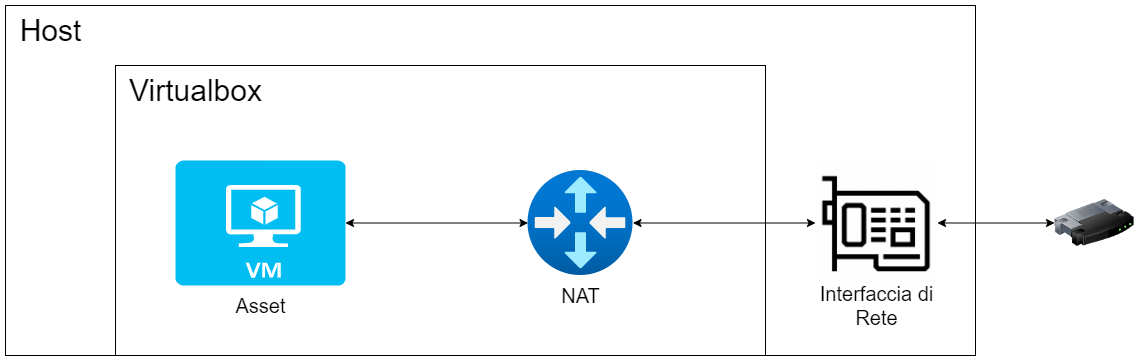
\includegraphics[scale=0.3]{capitoli/figure/schema-rete-nat-solo-asset.png}
    \caption{Infrastruttura di rete}
\end{figure}


\section{Strumenti utilizzati}
Per proseguire con l'analisi dell'asset, è necessario ottenere strumenti appositi che permettono di realizzare scansioni, mapping di vulnerabilità, ecc. Visto che, come già detto in precedenza, l'asset è una \emph{macchina virtuale} che sarà eseguita in un \emph{ambiente di virtualizzazione} e all'interno di una \emph{rete virtuale con NAT}, il modo più semplice per analizzare l'asset è quella di utilizzare una macchina virtuale realizzata apposta per questo scopo. A tal proposito, si è scelto di utilizzare una macchina virtuale molto popolare chiamata \textbf{Kali Linux} (in particolare la versione di riferimento \textbf{2023.1}) che viene distribuito con una suite di strumenti pronti all'uso per effettuare attività di Penetration Testing, Digital Forensics e altre simili. A questo punto, essendo che anche \textbf{Kali Linux} è una macchina virtuale che viene eseguita all'interno di \emph{VirtualBox}, verrà configurata anch'essa in modo tale che si colleghi alla \emph{rete con NAT} creata in precedenza. Otteniamo così il seguente schema:

\begin{figure}[h]
    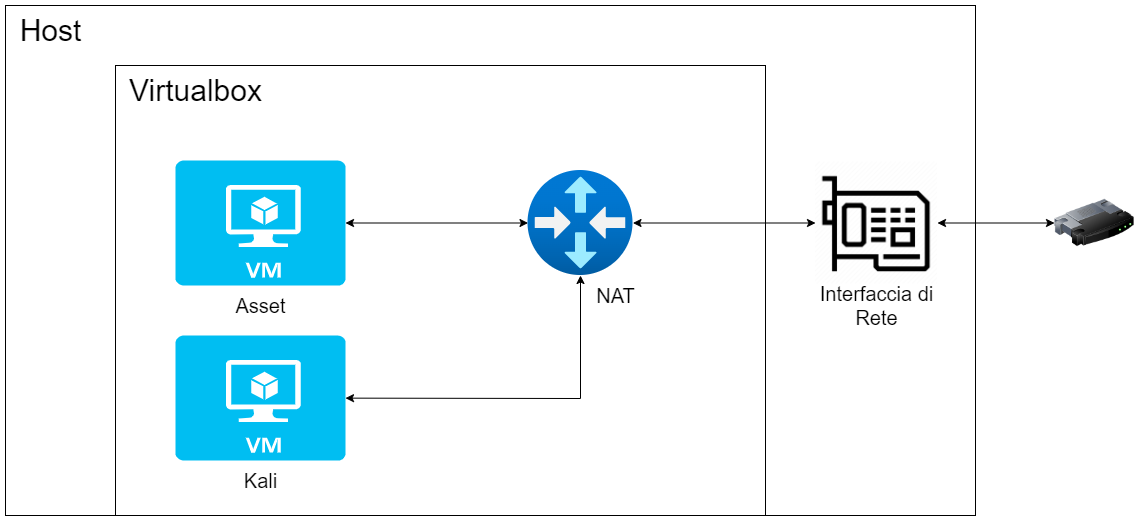
\includegraphics[scale=0.25]{capitoli/figure/schema-rete-nat-kali.png}
    \caption{Infrastruttura di rete con Kali}
\end{figure}

%\part{Impatto ambientale}

\backmatter
%*******************************************************
% Bibliografia
%*******************************************************
\cleardoublepage
\phantomsection
\addcontentsline{toc}{chapter}{\bibname}
\nocite{*}
\bibliographystyle{classic}
\bibliography{bibliografia}
%


\end{document}
